\documentclass[12pt]{extarticle}
%Some packages I commonly use.
\usepackage[portuguese]{babel}
\usepackage{graphicx}
\usepackage{framed}
\usepackage[normalem]{ulem}
\usepackage{amsmath}
\usepackage{amsthm}
\usepackage{amssymb}
\usepackage{amsfonts}
\usepackage{enumerate}
\usepackage[utf8]{inputenc}
\usepackage{float}
\usepackage{gensymb}
\usepackage[top=1 in,bottom=1in, left=1 in, right=1 in]{geometry}
\usepackage{multirow}
\usepackage{caption}
\usepackage{subcaption}
\usepackage[utf8]{inputenc}
\usepackage{tikz}

%A bunch of definitions that make my life easier
\newcommand{\matlab}{{\sc Matlab} }
\newcommand{\cvec}[1]{{\mathbf #1}}
\newcommand{\rvec}[1]{\vec{\mathbf #1}}
\newcommand{\ihat}{\hat{\textbf{\i}}}
\newcommand{\jhat}{\hat{\textbf{\j}}}
\newcommand{\khat}{\hat{\textbf{k}}}
\newcommand{\minor}{{\rm minor}}
\newcommand{\trace}{{\rm trace}}
\newcommand{\spn}{{\rm Span}}
\newcommand{\rem}{{\rm rem}}
\newcommand{\ran}{{\rm range}}
\newcommand{\range}{{\rm range}}
\newcommand{\mdiv}{{\rm div}}
\newcommand{\proj}{{\rm proj}}
\newcommand{\R}{\mathbb{R}}
\newcommand{\N}{\mathbb{N}}
\newcommand{\Q}{\mathbb{Q}}
\newcommand{\Z}{\mathbb{Z}}
\newcommand{\<}{\langle}
\renewcommand{\>}{\rangle}
\renewcommand{\emptyset}{\varnothing}
\newcommand{\attn}[1]{\textbf{#1}}
\theoremstyle{definition}
\newtheorem{theorem}{Theorem}
\newtheorem{corollary}{Corollary}
\newtheorem*{definition}{Definition}
\newtheorem*{example}{Example}
\newtheorem*{note}{Note}
\newtheorem{exercise}{Exercise}
\newcommand{\bproof}{\bigskip {\bf Proof. }}
\newcommand{\eproof}{\hfill\qedsymbol}
\newcommand{\Disp}{\displaystyle}
\newcommand{\qe}{\hfill\(\bigtriangledown\)}
\setlength{\columnseprule}{1 pt}
\usepackage[utf8]{inputenc}

\usetikzlibrary{arrows,shapes,positioning,angles}
\usetikzlibrary{decorations.markings}
\tikzstyle arrowstyle=[scale=1]

\title{Aula 27 - Equilíbrio estático e dinâmico}
\author{Felipe Salvador}
\date{Atualizado em \today}

\begin{document}

\maketitle

\section{Introdução}
Nessa aula, iremos estudar a parte sobre equilíbrio estático e dinâmico e como funciona o equilíbrio de forças sobre um corpo. Construíremos uma forma de como analisar os problemas e como resolvê-los. Ao final, trataremos sobre a estabilidade do equilíbrio.

\section{Análise do Equilíbrio}
Os estudos de estática são somente sobre os \textbf{corpos extensos} (corpos em que o seu formato e tamanho importam para o problema e não pode ser desconsiderado). Por isso, analisar as forças atuando um corpo deve ser feita de forma cautelosa, pois dependendo da posição em que a força é aplicada, o corpo faz um movimento diferente do que quando a posição de aplicação da força é outra.

Para sistemizar a análise, vamos definir uma quantidade chamada de \textbf{centro de massa (CM)}.

\subsection{Centro de Massa (CM)}

O centro de massa é um ponto no corpo onde se eu aplicar uma força, o corpo não rodará/rotacionará. É nesse ponto em que podemos reduzir um corpo extenso em caso problemas que não dependam/demandam da geometria do corpo. \textbf{O mais importante sobre o centro de massa é que não necessariamente ele coincide com o centro geométrico do objeto.} Ou seja, caso o objeto seja um cubo, dependendo de como a massa esteja espalhada pelo cubo, o centro de massa pode não coincidir com o centro geométrico do cubo (o meio dele).

Nós só iremos analisar os problemas de centro de massa de objetos em que a massa não é espalhada continuamente pelo corpo, ela está concentrada em pontos definidos, como um haltere.

Supondo um objeto trimensional que tenha massa em 2 pontos, cujas coordenadas e massa nesses pontos sejam $m_1$ em $(x_1,y_1,z_1)$ e $m_2$ em $(x_2,y_2,z_2)$, as coordenadas do centro de massa $(x_{CM},y_{CM},z_{CM})$ são:
\begin{equation}
    \begin{split}
        x_{CM} &= \frac{x_1\,m_1 + x_2\,m_2}{m_1+m_2}\\
        y_{CM} &= \frac{y_1\,m_1 + y_2\,m_2}{m_1+m_2}\\
        z_{CM} &= \frac{z_1\,m_1 + z_2\,m_2}{m_1+m_2}
    \end{split}
\end{equation}

Isso pode ser extrapolado para um número genérico finito $n$ de pontos que tenham massa:
\begin{equation}
    \begin{split}
        x_{CM} &= \frac{x_1\,m_1 + x_2\,m_2 + \dots + x_n\,m_n}{m_1+m_2+ \dots+ m_n}\\
        y_{CM} &= \frac{y_1\,m_1 + y_2\,m_2 + \dots + y_n\,m_n}{m_1+m_2+\dots+m_n}\\
        z_{CM} &= \frac{z_1\,m_1 + z_2\,m_2 + \dots + z_n\,m_n}{m_1+m_2+\dots+ m_n}
    \end{split}
\end{equation}

\textit{Obs:} \textbf{O nome Centro de Gravidade (CG) também é usado para indicar o Centro de Massa.} Normalmente ele é usado para quando estamos analisar problemas que envolvam a força peso $(\vec{P})$.

\subsection{Equilíbrio Estático e Dinâmico de Pontos Materiais}
Vamos analisar o equilíbrio para o caso mais simples: o caso em que o tamanho e a geometria do corpo não importa (quando o corpo é um ponto material).

A condição de equilíbrio para um ponto material é a seguinte:
\begin{equation}\label{eq:equilibrium}
    \vec{F}_R=\vec{F}_1 + \vec{F}_2 + \dots + \vec{F}_n = 0
\end{equation}
\noindent em que $\vec{F}_R$ é a força resultante e $n$ é o número de forças atuando no corpo. Ou seja, a soma vetorial de todas as forças agindo num corpo, que é um ponto material, é zero.

Podemos também analisar as forças nas direções $x$ e $y$. A condição de equilíbrio então:
\begin{equation}\label{eq:equilibrium_xy}
    \begin{split}
        &F_{1x} + F_{2x} + \dots + F_{nx} = 0\\
        &F_{1y} + F_{2y} + \dots + F_{ny} = 0\\
    \end{split}
\end{equation}

Vamos analisar um exemplo.

\begin{figure}[H]
    \centering
    \begin{tikzpicture}
         \coordinate (O) at (0,0);
         \coordinate (A) at (3,0);
         \coordinate (B) at (0,3);
         \coordinate (C) at (3,2);
         \coordinate (m) at (0,.2);
         
         \draw[black, thick, dash pattern=on 3pt off 3pt] (O) -- (A);
         \draw[black, thick, dash pattern=on 3pt off 3pt] (O) -- (B);
         \filldraw[black,fill=black!25!] (O) circle (5pt);
         \draw[black, thick, ->] (O) -- ++(1,2);
         \draw[black, thick, ->] (O) -- ++(0,-2);
         \draw[black, thick, ->] (O) -- ++(-1,0);
         \draw[black,thick] (O)+(0.75,0) arc (0:50:1);
         
         \path (O) ++(0,-2.3) node {$\vec{F}_1$};
         \path (O) ++(-1.3,0) node {$\vec{F}_2$};
         \path (O) ++(1.3,2.2) node {$\vec{F}_3$};
         \path (O) ++(0,3.2) node {$y$};
         \path (O) ++(3.2,0) node {$x$};
         \path (O) ++(.85,.6) node {$\theta$};
    \end{tikzpicture}
    \caption{Esquema das forças agindo num corpo em equilíbrio.}
    \label{fig:eq_ponto_material}
\end{figure}

Vemos que a força $\vec{F}_1$ e $\vec{F}_2$ estão nas direções $-y$ e $x$, respectivamente, e a força $\vec{F}_3$ está numa combinação dessas 2 direções. Iremos analisar as forças nas direções $x$ e $y$, então devemos decompor $\vec{F}_3$ nessas direções:
\begin{equation}
    \begin{split}
        &F_{3x} = F_3\,\cos\theta\\
        &F_{3y} = F_3\,sen\, \theta
    \end{split}
\end{equation}
Então:
\begin{align*}
    &-F_2 + F_3\,\cos\theta =0\quad\quad\text{na direção x}\\
    &-F_1 + F_3\,sin\,\theta=0\quad\quad\text{na direção y}
\end{align*}
Temos 4 quantidades ($F_1,\,F_2,\,F_3,\,\theta$) e sabendo 3 dessas, podemos determinar a quarta resolvendo esse sistema.
Importante ressaltar que nós podemos escolher as direções dos eixos $x$ e $y$, de preferência que eles sejam perpendiculares. Essa escolha pode facilitar a resolução do problema, como no caso do plano inclinado, em que escolhendo as direções de descida e a direção perpendicular ao plano facilitam as contas. 

\textbf{Caso haja forças que não estejam alinhadas a um dos eixos, temos que decompor a força tomando o ângulo $\theta$ como o ângulo entre a força e o eixo x.}

\subsection{Torque ($\vec{M}$)}
O torque é uma quantidade física análoga à força, mas que é utilizada quando analisamos um corpo extenso está sujeito à rotação. Uma questão importante é que o torque é o responsável por fazerem corpos rodarem e que, não necessariamente, o torque e a força possuem o mesmo valor. Há casos que a força tem um valor, mas o torque é zero, logo o corpo não será forçado a rodar.

O torque é definido como:
\begin{equation}
    M = F\,d\, sen \theta
\end{equation}
\noindent em que $F$ é a força aplicada, $d$ é o comprimento do braço de alavanca e $\theta$ é o ângulo entre a força e o braço de alavanca. Braço de alavanca é a distância entre o ponto em que a força é aplicada e um ponto do objeto é fixo (não se move).

\begin{figure}[H]
    \centering
    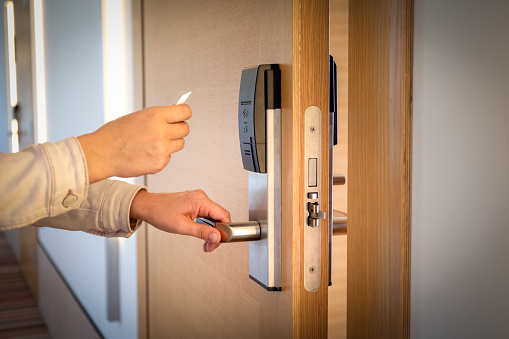
\includegraphics[width=0.6\textwidth]{porta.jpg}
    \caption{Imagem de uma porta. A razão pela qual a maçaneta está no extremo de fora da porta é que, para gerar um torque que faça a porta abrir, a força necessária é bem pequena porque o braço de alavanca é grande (nesse caso é a distância entre a dobradiça e a maçaneta)}
    \label{fig:porta}
\end{figure}

É por causa do torque que chaves de fenda, chaves inglesas são longas de forma que o braço de alavanca seja grande. Assim, para fazer o parafuso rodar, a força necessária não precisa grande para que o torque seja grande.

\textbf{Em caso de um corpo solto (sem que uma parte dele esteja preso), o braço de alavanca será a distância entre o ponto de aplicação da força e um ponto de referência chamado Pólo. Podemos escolher esse ponto de referência, mas uma vez escolhido, usamos ele até o final do exercício. Na maioria das vezes, é mais vantajoso escolher o pólo no ponto do Centro de Massa (CM), pois, caso tenhamos forças aplicadas no centro de massa (CM), elas não fazem rodar o corpo extenso: o torque aplicado será sempre 0.}
Assim, tiramos um torque do problema, assim fazemos menos contas.

Um exemplo de força que atua sempre no centro de massa é a força peso ($\vec{P}$).

\begin{figure}[H]
    \centering
    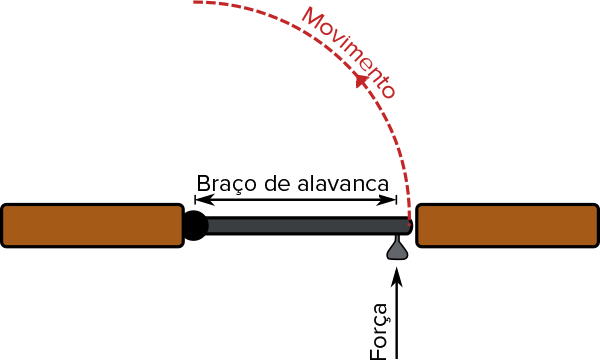
\includegraphics[width=0.6\textwidth]{torque.png}
    \caption{Diagrama das quantidades do torque. O braço de alavanca é a distância do ponto de aplicação da força até a dobradiça.}
    \label{fig:torque_porta}
\end{figure}

\subsection{Equilíbrio em corpos extensos}

Vamos analisar o caso do equilíbrio para um corpo extenso. A condição do equilibrio, que vimos para ponto material, continua a mesma:
\begin{equation}
    \vec{F}_R=\vec{F}_1 + \vec{F}_2 + \dots + \vec{F}_n = 0 \tag{\ref{eq:equilibrium}}
\end{equation}
Ou
\begin{equation}
    \begin{split}
        &F_{1x} + F_{2x} + \dots + F_{nx} = 0\\
        &F_{1y} + F_{2y} + \dots + F_{ny} = 0\\
    \end{split}
    \tag{\ref{eq:equilibrium_xy}}
\end{equation}

Mas isso não contempla todos os tipos de equilíbrio, pois o corpo pode girar. Caso imposermos que o nosso corpo extenso não gire, precisamos de outra condição: 
\begin{equation}\label{eq:torque_equilibrio}
    \vec{M}_R=\vec{M}_1 + \vec{M}_2 + \dots + \vec{M}_n=0
\end{equation}
\noindent em que $n$ é o número de torques aplicados ao corpo. Essas 2 condições (\ref{eq:equilibrium}) e (\ref{eq:torque_equilibrio}) são necessárias para que um corpo extenso esteja no equilíbrio, em que ele não gire.

Porém, há casos em que o corpo está em equilíbrio (eq. (\ref{eq:equilibrium}) é satisfeita), mas a equação (\ref{eq:torque_equilibrio}) não é satisfeita, ou seja, o torque resultante (lado esquerdo da eq. (\ref{eq:torque_equilibrio})) não é zero. Então, esse corpo ficará num certo espaço, mas rodando cada vez mais rápido.

Esse tipo de equilíbrio é chamado de \textbf{binário}, pois demanda de um par de forças que atuam em sentidos opostos e aplicadas em pontos diferentes do que o centro de massa. 

Na maioria dos casos, queremos um equilíbrio translacional (eq. (\ref{eq:equilibrium})) e também um equilíbrio rotacional (eq. (\ref{eq:torque_equilibrio})). Normalmente, o último é o mais difícil de ser satisfeito no caso da engenharia civil e mecânica na construção de pontes, edifícios e obras em que haja um vão livre bem grande. Se o torque resultante não for zero, o prédio poderá colapsar e implodir.

\subsection{Tipos de Equilíbrio}
Ao todo temos 3 tipos de equilíbrio:
\begin{itemize}
    \item \textbf{Equilíbrio estável} - quando um objeto é tirado da posição de equilíbrio, ele retorna de volta para ela. Ex: \textit{bola dentro de um buraco.}
    \item \textbf{Equilíbrio instável} - quando um objeto é tirado da posição de equilíbrio, ele nunca mais volta para ela. Ex: \textit{uma bola no topo de uma montanha}.
    \item \textbf{Equilíbrio indiferente} - quando mexemos no objeto, a nova posição do objeto é a posição de equilíbrio
\end{itemize}

\begin{figure}[H]
    \centering
    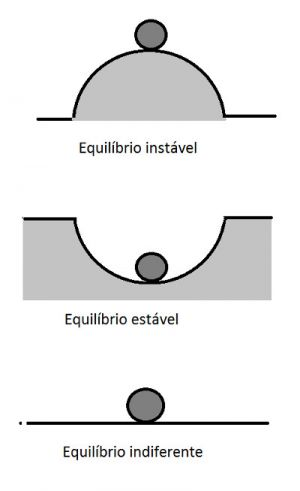
\includegraphics[width=0.4\textwidth]{tipos-de-equilibrio_300x491.jpg}
    \caption{Diagrama com os tipos de equilíbrio}
    \label{fig:tipos_de_equilibrio}
\end{figure}
\end{document}
